\documentclass[a4paper,10pt]{article}

\usepackage[english,french]{babel}
\usepackage[utf8x]{inputenc}
\usepackage[T1]{fontenc}
\usepackage{bookman}
\usepackage{amsmath}
\usepackage{amscd}
\usepackage{amssymb}
\usepackage{amsthm}
\usepackage{latexsym}
\usepackage{graphicx}
\usepackage{color}
\usepackage{calc}
\usepackage{setspace}
\usepackage[boxruled,vlined,french]{algorithm2e}
% \usepackage{CJK}

\setlength{\voffset}{-3.75cm}
\setlength{\hoffset}{-2.6cm}
\setlength{\oddsidemargin}{2.75cm}
\setlength{\topmargin}{2in}
\setlength{\headheight}{0in}
\setlength{\headsep}{0in}
\setlength{\topskip}{0in}
\setlength{\parindent}{0cm}
\setlength{\parskip}{1ex plus0.4ex minus0.2ex}
\setlength{\textwidth}{16.25cm}
\setlength{\textheight}{20.5cm}
\renewcommand{\baselinestretch}{1.5}
\flushbottom
\setcounter{page}{1}
\setcounter{tocdepth}{2}

\SetKw{Edb}{Effet de bord}
\SetKw{Et}{et}
\SetKw{Ou}{ou}
\SetKw{De}{de}
\SetKw{A}{à}
\SetKwBlock{Debut}{Début}{Fin}
\SetKwIF{Si}{SinonSi}{Sinon}{Si}{alors}{Sinon si}{Sinon}{FinSi}
\SetKwFor{Pour}{Pour}{faire}{FinPour}
\SetKwFor{PourTout}{Pour tout}{faire}{FinPour}
\SetKwFor{TantQue}{Tant que}{faire}{FinTantQue}
\SetKw{Retour}{retourner}

\newcommand{\anym}{\emph{anymalign}}
\newcommand{\guill}[1]{«~#1~»}

\newtheorem{probleme}{Problème}


% $$$ Faire une Titlepage un peu plus jolie...
\title{ \Large Rapport de stage \\ \LARGE Analyse d'un algorithme d'alignement multilingue}

\author{\normalsize Romain \textsc{Versaevel}, L3 Informatique Fondamentale, ENS de Lyon \\ \normalsize Encadré par M. François \textsc{Yvon}, directeur du LIMSI/CNRS \\}

\date{\today}

\begin{document}

\maketitle

\begin{abstract}
Ce rapport rend compte de mon stage de Licence 3 réalisé au LIMSI/CNRS, durant lequel j'ai étudié l'algorithme d'alignement multilingue \anym .

Après une présentation du domaine de recherche, le traitement automatique des langues parlées, et plus particulièrement la traduction automatique, je propose les résultats pratiques et théoriques de mon analyse. Ceux-ci valident l'algorithme \anym~et en montrent certaines limites à travers la comparaison avec des mesures d'association et des calculs de probabilités.
\end{abstract}

\newpage
\tableofcontents
\newpage

\section{Introduction}
J'ai suivi dans le cadre de ma formation, en Licence 3 d'Informatique à l'ENS de Lyon un stage de recherche d'une durée de six semaines, du 2 juin au 11 juillet 2014. Ce stage s'est déroulé au LIMSI (Laboratoire d'Informatique pour la Mécanique et les Sciences de l'Ingénieur), laboratoire CNRS situé sur le campus de l'université Paris-Sud, à Orsay, dans le groupe TLP (Traitement des Langues parlées, ou Spoken Language Processing Group). J'étais encadré par M. François Yvon, chercheur au LIMSI, animateur du thème \guill{Traduction automatique}.

Le sujet de ce stage était d'analyser l'algorithme d'alignement multilingue \anym, conçu et implémenté par Adrien Lardilleux
% £££
en
% £££
, disponible sur \cite{anymalign}, et utilisé par le LIMSI pour diverses applications.

Ce rapport est divisé en quatre parties. Dans la première, je présente le contexte dans lequel s'inscrit mon travail, le domaine de la traduction automatique. Dans la deuxième, je présente l'algorithme que j'ai étudié et l'analyse qui en avait déjà été réalisée. Dans les troisième et quatrième, je présente les résultats de ma propre analyse, empirique (confrontation avec des mesures d'association) et théorique.



\section{Contexte, rappels}

Cette section présente le domaine de recherche dans lequel s'inscrit mon stage : le traitement automatique des langues parlées, puis plus particulièrement la traduction automatique. Elle est essentiellement bibliographique.

\subsection{Traitement des langues parlées}

Le traitement automatique des langues parlées, en anglais \emph{spoken language processing} (ou encore linguistique automatique, \emph{computational linguistics}) est une discipline à l'intersection de l'informatique, de la linguistique, des sciences cognitives. Son objet est l'étude et l'utilisation des langues naturelles avec des outils informatiques.

Ses applications sont nombreuses. On peut citer le traitement du signal pour la synthèse et la reconnaissance vocale, les interfaces homme/machine, l'écriture automatique %article du Monde
, et la traduction automatique.



\subsection{Traduction automatique}

La \emph{traduction automatique}, en anglais \emph{machine translation}, a pour objet la traduction de textes d'une langue naturelle vers une autre, par l'intermédiaire d'algorithmes et d'ordinateurs (sans intervention humaine --- on parle sinon de \emph{traduction assistée par ordinateur}). Si l'on peut chercher les origines de cette discipline dans les langues universelles imaginées par Descartes et Leibniz au XVII\textsuperscript{e} siècle
\footnote{Dans respectivement la \emph{Lettre au P. Mersenne} du 20 novembre 1629
(1) Edition Clerselier, t. I, no. 111, p. 498; éd. Cousin, t. VI, p. 61; éd. Adam-Tennery, t. I, p. 76 (Paris, Cerf, 1898).
et \emph{Dissertatio de arte combinatoria}}
, par le truchement desquelles on pourrait passer de n'importe quelle langue à n'importe quelle autre, c'est en 1947 que le mathématicien américain Warren Weaver propose pour la première fois d'utiliser les ordinateurs pour réaliser des travaux de traduction à l'UNESCO (dans une lettre à Norbert Wiener : \cite{weaver1947letters}).
La discipline a depuis fait des progrès considérables. Ses motivations, développées par John Hutchins dans \cite{hutchins1986machine}, 
sont nombreuses. Hutchins évoque la nécessité dans certaines professions de consulter des documents rédigés dans des langues très diverses, la simplification de la transmission des savoirs, des applications militaires, mais aussi des raisons plus idéologiques : la traduction permet la communication et donc la paix. Notons que la traduction automatique ne fait pas concurrence aux traducteurs humains, qui s'adressent à un public différent. Sa vocation n'est pas de réaliser des traductions littéraires ou des traductions parfaites, mais de rendre accessible, rapidement et à moindre coût, une très grande quantité de documents à des locuteurs de toutes les langues.

La traduction est un exercice considéré difficile depuis longtemps. \guill{Traduttore, traditore} disent les italiens : \guill{Traduire, c'est trahir}. Les ordinateurs n'ont pas des prétentions si élevées que celle de transmettre fidèlement la pensée de l'auteur original ; ils doivent cependant relever toutes sortes de défis. Ainsi l'idée naïve d'une traduction mot à mot à l'aide d'un simple dictionnaire bilingue produit-elle de très mauvais résultats, parce qu'un mot dans une langue peut se traduire par plusieurs dans une autre (\emph{Rindfleischetikettierungsüberwachungsaufgavenübertragungsgesetz} est ainsi l'équivalent allemand de \emph{loi sur le transfert des obligations de surveillance de l'étiquetage de la viande bovine} en français, soit 1 mot contre 15), parce que la polysémie ou l'homonymie ne sont pas prises en compte (faut-il traduire \emph{avocat} par \emph{avocado} ou \emph{lawyer} ? \emph{cut} par \emph{couper}, par \emph{coupé}, par \emph{coupions} ?), non plus que les idiomes (\emph{Das ist nicht mein Bier} doit être traduit par \emph{Ce ne sont pas mes oignons} et non littéralement par \emph{Ce n'est pas ma bière}), etc.

Bon nombre d'outils de traduction automatique ont été développés, les plus connus étant Google translate et SYSTRAN (utilisé par Yahoo et BabelFish). Les approches sont nombreuses, elles peuvent s'appuyer ou non sur des outils d'analyse linguistique, être orientées (distinguer les rôles des langues \emph{source} et \emph{destination}) ou symétriques, statistiques ou non\dots
% Liens ; statistiques ? £££

Les algorithmes qui nous intéressent plus particulièrement ici ne sont pas des algorithmes de traduction pure mais des algorithmes d'\emph{alignement}, qui génèrent des données pour les premiers en analysant des corpus édités en plusieurs langues. On cite souvent l'exemple de Champollion qui apprit à déchiffrer les hiéroglyphes grâce à la pierre de Rosette. Les algorithmes d'alignement utilisent ainsi des corpus multilingues --- dont il existe grâce à Internet de grandes quantités --- pour en extraire des relations de traduction entre des paires de mot ou groupes de mots. Les modèles les plus répandus sont les modèles IBM, numéroté de 1 à 6 (\cite{vogel1996hmm} et \cite{och2003systematic}) dont Giza++ \cite{och2003giza++} implémente les algorithmes d'estimation et de décodage. On peut encore citer le Berkeley Word Aligner (\cite{berkeleywordaligner}), Nile (\cite{nilewordaligner}). Pour plus d'informations sur la traduction automatique statistique, voir \cite{Brown:1990:SAM:92858.92860} et \cite{gaussier2011modeles}.

Remarquons que le mot \guill{alignement} sera régulièrement utilisé de manière abusive dans ce document ; il a été introduit par analogie avec le fonctionnement des \emph{algorithmes d'alignement} les plus répandus ; mais il ne décrit pas vraiment le comportement d'\anym.

\subsection{Quelques définitions et notations}

\subsubsection{Langues naturelles}

Avant d'étudier plus avant \anym, il convient de poser quelques définitions.

Dans un texte en langue naturelle, on appelle \emph{segment} (\emph{phrase} en anglais) une séquence de mots adjacents. On appellera en outre $n$-gram un segment de $n$ mots consécutifs.

On appelle \emph{corpus multilingue} un ensemble de textes en plusieurs langues. On appelle \emph{corpus parallèle} un corpus multilingue dont les textes sont traduction les uns des autres. Enfin, un corpus parallèle est \emph{aligné} lorsque sont déterminées des relations (de traduction) entre segments de ses textes.

\anym~considère des corpus parallèles de taille arbitraire alignés au niveau des phrases, et construit de manière non-orientée un dictionnaire d'alignements de segments plus petits. On limitera ici notre analyse à des corpus de deux seulement textes, qu'on appellera \emph{texte source} et \emph{texte cible}.
% ; un mot ou segment du texte source sera généralement noté $e$ (comme \emph{english}) et du texte cible $f$ (comme \emph{french} ou \emph{foreign})




\subsubsection{Fréquences des mots}

\label{zipf}

Les fréquences des mots dans les langues naturelles traitées joue naturellement un rôle important dans le comportement de l'algorithme. On considérera qu'elles suivent la \emph{loi empirique de Zipf} (introduite dans \cite{zipf1935psycho} et dans \cite{zipf1949human})
: si l'on classe les mots du corpus par fréquence décroissante, la fréquence $f$ d'un mot est liée au rang $n$ de ce mot par $f = \frac{K}{n}$ (avec $K$ une constante). On se contentera ici de cette version empirique ; pour plus de détails sur cette loi, en particulier ses variantes mathématiques permettant de définir une fonction de masse (impossible sous cette formulation à cause de la divergence de la série harmonique), se référer à \cite{baayen2001word}. Selon la loi de Zipf , la langue contient quelques mots-outils très fréquents (en français les mots les plus fréquents sont \guill{de}, \guill{la}, \guill{le}, \guill{un}, etc.) et des mots rares mais nombreux (ainsi de la plupart des mots porteurs de sens : substantifs, adjectifs, verbes, adverbes). Remarquons que ce modèle convient bien aux langues alphabétiques, mais n'est pas adapté pour décrire d'autres systèmes, par exemple ceux employant des logogrammes (hiéroglyphes, chinois mandarin\dots).

Enfin, on appelle \emph{hapax} un mot qui apparaît une seule fois dans un corpus  \footnote{La Bible comporte entre 1000 et 2000 hapax.}



\section{Présentation d'\emph{anymalign}}

Dans cette partie, je présente l'algorithme \anym, donne un aperçu de son fonctionnement, et présente les principaux résultats déjà publiés à son sujet.

\subsection{L'algorithme}

L'aglorithme \ref{algoanym} décrit le comportement général d'\anym.

\begin{algorithm}
\setstretch{1.5}
\caption{anymalign \label{algoanym}}
\SetKwData{Cu}{C$_1$} \SetKwData{Cn}{C$_n$} \SetKwData{Wu}{w$_{n_1}$} \SetKwData{Wn}{w$_{n_k}$} \SetKwData{AlC}{Table} \SetKwData{iii}{i} \SetKwData{jjj}{j} \SetKwData{www}{w} \SetKwData{J}{J} \SetKwData{I}{I} \SetKwData{Sub}{S} \SetKwData{Profils}{Profils} \SetKwFunction{ajouter}{ajouter} 

\Entree{Corpus parallèle $(\Cu, \dots, \Cn)$.}
\Sortie{Table d'alignements \AlC.}

\Debut
{
	\Pour{\iii de $1$ à \I}
	{
		\Sub $\leftarrow$ sous-corpus de taille $|\Sub|$

		\Pour{\jjj de $1$ à \J}
		{
			\PourTout{\jjj-gram \www dans \Sub}
			{
				Calculer son profil (vecteur de présence) \\
				\ajouter$(\www,\Profils)$
			}

			\PourTout{$\pi$ dans \Profils}
			{
				$(\Wu,\dots,\Wn) \longleftarrow$ mots de profil $\pi$ \\
				$\AlC[(\Wu,\dots,\Wn)]$ ++
			}
		}
	}
	\Retour \AlC
}
\end{algorithm}

La fonction auxiliaire $ajouter$ incorpore le mot $w$ dans la table $Profils$, initialement vide, de telle sorte que :

\begin{itemize}
\item si $Profils$ contient déjà $w'\subset w$ de même profil que $w$, alors $w'$ est écrasé par $w$ ;
\item si plusieurs segments d'un même texte ont le même profil, ils sont finalement tous rejetés.
\end{itemize}

\subsubsection{Exemple}

Voici un exemple d'exécution de l'algorithme.

Supposons que le sous-corpus tiré aléatoirement contienne les phrases suivantes :

\begin{tabular}{|c|l|l|}
\hline
\dots & \dots & \dots \\
10 & L' avocat fumait au zoo . & The lawyer smoked in the zoo . \\
11 & En entrée : salade d' avocat . & Starter : avocado salad . \\
12 & Les singes au zoo mangent de l' avocat . & Monkeys in the zoo eat avocado . \\
\dots & \dots & \dots \\
\hline
\end{tabular}

\`A l'étape des $1$-grams, le calcul des profils aboutit au tableau suivant :

\begin{tabular}{|c|c|c|c|c|c|c|c|c|c|c|}
\hline
avocat & zoo$_{fr}$ & singes & .$_{fr}$ & \dots & lawyer & avocado & zoo$_{en}$ & Monkeys & .$_{en}$ & \dots \\
\hline
1 & 1 & 0 & 1 & \dots & 1 & 0 & 1 & 0 & 1 & \dots \\
1 & 0 & 0 & 1 & \dots & 0 & 1 & 0 & 0 & 1 & \dots \\
1 & 1 & 1 & 1 & \dots & 0 & 1 & 1 & 1 & 1 & \dots \\
\hline
\end{tabular}

Ainsi, on pourra incrémenter $Table[zoo_{fr},zoo_{en}]$ et $Table[singes,Monkeys]$. En revanche, la présence de deux traductions différentes d'$avocat$ empêche de l'aligner. Faute de plus d'informations, on ne le distingue d'ailleurs pas de $._{fr}$ en français. Les autres phrases pourraient permettre de faire apparaître $fumait-smoked$, $entrée-starter$, $salade-salad$ \dots~comme des \guill{hapax locaux}, et d'incrémenter leur score.

\`A l'étape des $2$-grams, $au~zoo$ et $the~zoo$, de profil $(1,0,1)$, remplaceront $zoo_{fr}$ et $zoo_{en}$ dans le tableau $Profils$, et seront alignés. \`A celle des $3$-grams, $in~the~zoo$ écrasera à nouveau $the~zoo$ et sera aligné avec $au~zoo$.

Si $J$ a été paramétré suffisamment grand, des phrases entières pourront être alignées (par exemple la phrase 10, composée respectivement de 6 et 7 mots).



\subsubsection{Remarques}

Tel que présenté ici, l'algorithme termine après $I$ itérations ; en réalité, dans l'implémentation qui en a été faite, de nombreuses conditions d'interruption différentes peuvent être utilisées : après un certain temps, lorsque le nombre d'alignements par secondes devient inférieur à une certain borne, ou encore par une interruption manuelle de l'utilisateur.

Cette implémentation propose en outre de paramétrer les longueurs minimale et maximale des $n$-gram, ainsi que d'activer ou non l'alignement de  $n$-gram discontinus (par exemple \guill{ne $\_$ pas} dans \guill{ne t'en fais pas}). L'approche consiste alors, lorsqu'on incrémente le score des segments $e-f$ issus des phrases $E$ et $F$, d'incrémenter aussi celui de $(E\textbackslash e)-(F\textbackslash f)$. Même si on la trouve dans la description faite par \cite{lardilleux2013generalizing}, cette option est par défaut désactivée et je ne l'ai jamais utilisée.

\anym~est comme on le voit un algorithme statistique, dont l'exécution ne dépend pas de la taille du corpus ; il  utilise les seuls textes parallèles (et aucune donnée linguistique) ; c'est en outre un algorithme complètement symétrique : tous les corpus $C_i$ jouent le même rôle. Pour cette raison, on peut se contenter pour l'analyse de deux corpus $C_1$ et $C_2$, mais il s'agit évidemment d'une qualité importante de l'algorithme.


\subsection{Qualités et défauts}

Cette partie propose l'analyse d'\anym~telle qu'elle avait déjà été réalisée, dans \cite{lardilleux2013generalizing}.

La première évaluation consistait à comparer les paires de segments extraits par \anym~ et MGIZA++ (pendant la même durée) avec un dictionnaire bilingue de référence (ne contenant que les mots présents dans le corpus traité). Les résultats sont qu'\anym~couvre une plus grande partie de ce dictionnaire, en moyenne 7\%~de plus que MGIZA++ ; en revanche, ce dernier couvre bien plus de $n$-gram ($n\geq2$).

Ce phénomène s'explique par les difficultés qu'a \anym~produit très peu d'alignements de segments contenant à la fois des mots fréquents et des mots rares. En effet, les mots fréquents ne peuvent être correctement alignés qu'à travers des sous-corpus de petite taille, tandis que les mots rares en nécessitent de plus longs. En effet, lorsque la taille du corpus échantillonné augmente, il en va du même du risque que les mots fréquents apparaissent dans des usages différents (typiquement, que \guill{the} soit traduit par \guill{le} et par \guill{la}), tandis que cela révèle la rareté des mots rares ; les mots fréquents agissent alors comme un masque qui permet d'aligner facilement les mots rares, dont les petits profils sont faciles à identifier.

D'ailleurs, le résultat suivant est qu'\anym~a des performances supérieurs à MGIZA++ pour les mots rares (de $1$ à $5000$ occurrences dans un corpus de $30$ millions de mots) et inférieures sur les mots fréquents (plus de $5000$ occurrences). Si les seconds jouent les rôles les plus importants pour la traduction, les premiers sont les plus nombreux (voir la section \ref{zipf} sur la loi de Zipf).

Enfin, les résultats d'\anym~sont évalués par différentes métriques spécialisées (BLEU, TER) qui donnent des scores proches de ceux de MGIZA++, et des scores meilleurs pour l'utilisation combinée des deux algorithmes.

Les principales qualités d'\anym~mises sont les suivantes :
\begin{itemize}
\item l'algorithme est totalement  multilingue : il autorise l'utilisation d'un corpus d'entrée avec de nombreuses langues différentes ;
\item il est insensible à l'ordre des mots et donc aux inversions ;
\item il permet l'alignement de $n$-grams (ainsi \anym~identifiera que \guill{Victor Hugo} est la traduction de \guill{Victor Hugo}, sans avoir besoin de savoir que \guill{Victor} traduit \guill{Victor} et \guill{Hugo} \guill{Hugo}) ;
\item il est simple, et sa complexité algorithmique est maîtrisée.
\end{itemize}



\section{Mesures d'association}

Dans cette section, après avoir introduit la notion de \emph{mesure d'association} en statistiques, je compare les résultats empiriques fournis par \anym~avec différentes mesures d'association classiques.

\subsection{Définitions}

En statistiques, on appelle \emph{mesure d'association} une relation entre plusieurs variables aléatoires non-indépendantes. Le terme est proche de celui de \emph{corrélation} même si ce dernier a une définition plus contrainte, impliquant notamment d'un \emph{facteur de corrélation}.

En théorie de l'information, il s'agit le plus souvent de comparer deux variables aléatoires $X$ et $Y$. Notons $e$ et $f$ les événements $X \in E$ et $Y \in F$. Les mesures d'association entre $X$ et $Y$ utiliseront généralement les valeurs de la table de contingence ($\mathfrak{F}(e)$ désigne la fréquence absolue de l'événement $e$ dans un effectif de taille totale $N$) :

\begin{tabular}{|cc|c|}
\hline
$a := \mathfrak{F}(e\wedge f)$ & b := $\mathfrak{F}(e\wedge\overline{f})$ & $\mathfrak{F}(e)$ \\
$c := \mathfrak{F}(\overline{e}\wedge f)$ & $d := \mathfrak{F}(\overline{e}\wedge\overline{f})$ & $\mathfrak{F}(\overline{e})$ \\
\hline
$\mathfrak{F}(f)$ & $\mathfrak{F}(\overline{f})$ & $N$ \\
\hline
\end{tabular}

Ici, $X$ et $Y$ seront des mots ; $E$ et $F$ désigneront les phrases alignées d'un corpus parallèle de taille $N$. On mesurera donc l'association de deux mots à travers la probabilité qu'ils apparaissent dans une même phrase ($a$), le premier sans le deuxième ($b$), etc.

Le tableau suivant montre les mesures d'associations que j'ai utilisées. Elles proviennent de \cite{pecina2006combining}, qui présente un très grand nombre, et de \cite{hoang2009re} (qui exhibe des relations d'équivalence entre plusieurs mesures classiques, et m'a ainsi permis d'en éliminer certaines). % $$$ Le faire vraiment

Les mesures utilisées sont listées dans le tableau suivant (les noms sont donnés en anglais car certains n'ont pas d'équivalent français) :

\begin{tabular}{|l|l|}
\hline
Nom & Formule \\
\hline
Likelihood ratio ou $G^2$
% & $2\left(a\log\left(\frac{aN}{(a+b)(a+c)}\right) +b\log\left(\frac{bN}{(a+b)(b+d)}\right) +c\log\left(\frac{cN}{(a+c)(c+d)}\right) +d\log\left(\frac{dN}{(b+d)(c+d)}\right)\right)$ % ???

& $\sum_{x=e,\overline{e}}\sum_{y=f,\overline{f}}\mathfrak{F}(x\wedge y)\log\left(\frac{\mathfrak{F}(x\wedge y)}{\mathfrak{F}(x)\mathfrak{F}(y)}\right)$ \\

Pointwise % £££
 mutual information (PMI)  & $\log_2(\frac{aN}{(a+b)(a+c)})$ \\


$\Phi^2$ de Church \& Gale & $\frac{(ad-bc)^2}{(a+b)(a+c)(b+d)(c+d)}$ \\

Coefficient $Q$ de Yule & $\frac{ad-bc}{ad+bc}$ \\

Coefficient $\omega$ de Yule & $\frac{\sqrt{ad}-\sqrt{bc}}{\sqrt{ad}+\sqrt{bc}}$ \\

% Odds ratio & $\frac{ad}{bc}$ \\

Jaccard & $\frac{a}{a+b+c}$ \\

Normalized expectation & $\frac{2a}{2a+b+c}$ \\
%+redondant Jaccard? $$$

Salience & $\log\left(\frac{aN}{(a+b)(a+c)}\right)\cdot\log(a)$  \\
% redondant PMI? $$$

t test & $\frac{a-\frac{(a+b)(a+c)}{N}}{\sqrt{a(1-\frac{a}{N})}}$ \\

z score & $\frac{a-\frac{(a+b)(a+c)}{N}}{\sqrt{\frac{(a+b)(a+c)}{N}(1-\frac{(a+b)(a+c)}{N^2})}}$ \\

Braun-Blanquet & $\frac{a}{\max(a+b,a+c)}$ \\

Simpson & $\frac{a}{\min(a+b,a+c)}$ \\

Laplace & $\frac{a+1}{\min(b,c)+a+2}$ \\

\hline
\end{tabular}

On constate une grande diversité dans ces mesures, permise par la définition assez laxiste. Le principe est que la mesure est d'autant plus élevée que les les variables aléatoires sont dépendantes suivant un certain schéma. Notre objectif est de montrer que les paires de mots fréquemment alignées par \anym~ont une association forte. Il s'agit donc de comparer deux mesures d'association, puisque \anym~en réalise aussi une, quoique plus compliquée que les précédentes.

% on aimerait bien montrer que le rapport du nombre de fois qu'un couple de mots est aligné par le nombre d'itérations converge vers la probabilité que ce couple ait le même profil dans un sous-corpus tiré aléatoirement. ???

\subsection{Comparaison avec \anym}

Dans cette partie, on compare les résultats d'\anym~ avec les mesures d'association listées précédemment.

\subsubsection{\anym}

Ces résultats ont été obtenus en traitant un corpus français-anglais de 1000 lignes extrait du corpus \emph{Europarl} (\cite{koehn2005europarl}), contenant les compte-rendus de séances de la Commission Européenne dans une quinzaine de langues. L'exécution d'\anym~a été interrompue après de 2 200 000 itérations ; le nombre de nouveaux alignements par seconde était alors inférieur à 1 ; un peu plus de 45 000 paires de mots ont ainsi été alignées.

Les paires les plus alignées correspondent aux très fréquents, notamment les mots-outils et la ponctuation :

\begin{tabular}{|l|l|l|}
\hline
Français & Anglais & Nombre d'alignements \\
\hline
. & . & 6185271 \\
et & and & 394766 \\
je & I & 330634 \\
rapport & report & 329316 \\
Commission & Commission & 286020 \\
concurrence & competition & 277991 \\
\dots & \dots & \dots \\
\hline
\end{tabular}

Les alignements erronés les plus fréquents font eux aussi intervenir des mots-outils, présents dans une grande majorité des phrases ; le premier d'entre eux est (\guill{.},\guill{the}), au 103\textsuperscript{e} rang avec 25031 alignements.

1451 mots sont alignés plus de 1000 fois, 8266 mots plus 100 fois, 28264 mots plus de 10 fois.

Le critère de comparaison qui a été retenu pour comparer \anym~aux autres mesures d'association est le nombre d'alignements produits. D'autres ont été envisagées, notamment le \emph{score} calculé par \anym, qui correspond au nombre d'alignements divisé par la fréquence d'apparition des mots de la paire ; néanmoins il m'a paru moins pertinent lors de l'exploitation des graphiques qui apparaissent ci-après.

\subsubsection{Jaccard}

La mesure d'association dont les résultats m'ont paru les plus exploitables
est le Jaccard dont on rappelle l'expression : $Jacc(e,f)=\frac{a}{a+b+c}=\frac{\mathfrak{F}(e\wedge f)}{\mathfrak{F}(e\wedge f)+\mathfrak{F}(e\wedge\overline{f})+\mathfrak{F}(\overline{e}\wedge f)}$ ou, si l'on note $E$ (resp. $F$) l'ensemble des phrases où apparaît $e$ (resp. $f$) : $Jacc(e,f)=\frac{|E\cap F|}{|E\cup F|}$.

La figure \ref{jaccard} montre le nombre d'alignements % échelle log $$$
 réalisés par \anym~en fonction du Jaccard. On y observe une association importante : 
% Il faudrait peut-être étoffer ça d'une régression linéaire ? Je ne sais pas faire... ???
pour $j$ fixé, les couples de mots de Jaccard proche de $j$ les plus alignés le sont d'un nombre proche de $C\cdot j$ ($C$ une constante, de peu d'importance puisqu'elle dépend de la durée d'exécution de l'algorithme.) Ainsi, l'absence de points dans les coins supérieur gauche (les paires d'association faible sont peu alignées) et inférieur droit (les paires de forte association sont beaucoup alignées) valident l'algorithme. Tout à droite, les points de Jaccard $1$ correspondent aux traductions exactes (les paires de mots qui n'apparaissent jamais l'un sans l'autre). Précisons que pour des raisons de complexité, les hapax n'ont pas été pris en compte, qui apparaîtraient majoritairement à la même abscisse mais à des ordonnées inférieures.

En revanche, l'épaisseur de la courbe, en d'autres termes le grand nombre de points situés en-dessous de la courbe $y = C\cdot x$ montre une variation importante dans les alignements réalisés par \anym~pour des couples de mots de même Jaccard.
% quantifier ça... ???

\begin{figure}[t]
\centering
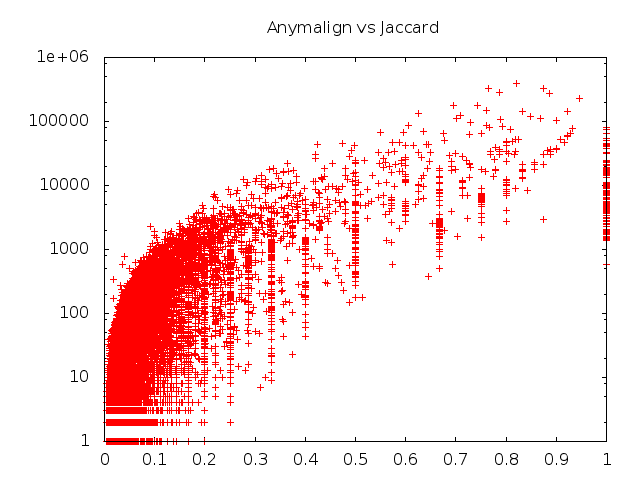
\includegraphics[width=12cm]{jacclog.png} % $$$ Penser à relooker (plus grand, échelle log au lieu de log, pas "../../moy/...")
\caption{Confrontation des résultats d'\anym~et du Jaccard}
\label{jaccard}
\end{figure}

Ces résultats montrent une ressemblance importante entre les résultats d'\anym~et le Jaccard ; l'algorithme en donne une estimation avec une complexité inférieure (le calcul du Jaccard de toutes les paires de mots d'un corpus de taille $N$ se fait en $O(N^2)$).
On aurait cependant espéré une proximité encore supérieure : la motivation de ces travaux se trouve dans l'article \cite{broder2000identifying}, où Broder fait apparaître le Jaccard pour valider ses techniques de \emph{min hashing} ; or celui-ci semblait dans son expression bien adapté pour décrire \anym.

D'autres mesures, pour lesquelles on trouvera les graphiques en annexe, donnent un résultat proche : il s'agit de Braun-Blanquet, Laplace, Normalized expectation, Simpson, et t test. % $$$

\subsubsection{PMI}
% Du coup je ne sais pas vraiment ce que c'est !!
% \log_2(Na/((a+b)(a+c))) = log_2(P(xy)/(P(x)P(y)))

Une autre mesure qui a retenu mon attention est l'Information Mutuelle (IM) % $$$
 dont on rappelle l'expression : $IM(e,f)=\log_2\left(\frac{aN}{(a+b)(a+c)}\right)=\log_2\left(\frac{\mathfrak{F}(e\wedge f)\cdot N}{\mathfrak{F}(e)\cdot\mathfrak{F}(f)}\right)$ (avec $N$ la taille totale du corpus).

La figure \ref{im} montre le nombre d'alignements % échelle log $$$
 réalisés par \anym~en fonction de l'Information Mutuelle.

\begin{figure}[t]
\centering
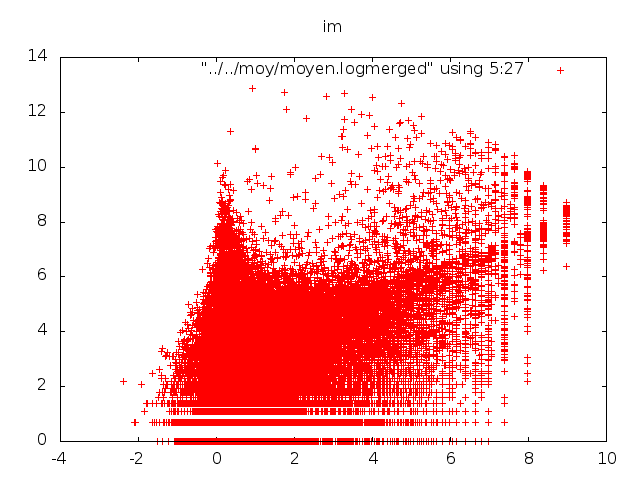
\includegraphics[width=12cm]{imlog.png} % $$$ Penser à relooker (plus grand, échelle log au lieu de log, pas "../../moy/...")
\caption{Confrontation des résultats d'\anym~et de l'Information Mutuelle}
\label{im}
\end{figure}

\textbf{Reste à faire un relooking des deux figures, et à ajouter quelques explications (échelle log).}

On observe une relation moins forte qu'avec le Jaccard. Cela est notamment lié au fait que l'Information Mutuelle dépend trop de la fréquence des mots (les mots rares auront systématiquement une Information Mutuelle plus élevée que les mots fréquents).

Les bons alignements entre mots fréquents apparaissent pour des IM comprises entre 1 et 4, et les mots rares équivalents pour les IM maximales ($log(N)=9,96$). Ainsi, la partie droite du graphique montre à nouveau qu'\anym~réalise une bonne mesure d'association.

Cependant, on observe aussi un pic autour de l'abscisse 0 et en-dessous, qui correspond à des paires de mots en faible relation. Ce pic fait apparaître les paires de mots alignées par erreur par \anym~(comme \guill{the} et \guill{.}). Ce qui a retenu mon attention avec cette mesure, c'est en effet que, sans invalider l'algorithme, elle montre que celui-ci produit une quantité importante de \guill{déchet}, en associant des paires de mots qui n'auraient pas dû être alignées.

Les autres mesures, pour lesquelles on trouvera également des graphiques en annexe, qui donnent des résultats proches sont Yule's omega, Yule's Q, et Salience.

\subsubsection{Conclusion}

La comparaison d'\anym~et de différentes mesures d'association a permis de valider encore une fois l'algorithme, en montrant qu'il réalisait une estimation proche du Jaccard, et à la fois d'en montrer une limite en révélant les mauvais alignements qu'il produit.

On trouvera en annexe les graphiques des autres mesures que j'ai essayées (le z score, le $\Phi^2$) mais qui ne m'ont pas semblé exploitables.

\section{Analyse théorique}

Dans cette partie, on cherche à analyser \anym~à l'aide de quelques calculs de probabilités.

La notion qu'il m'a paru intéressant d'étudier est celle de profil, qui est intrinsèquement liée au fonctionnement d'\anym. Je donne d'abord deux calculs de probabilités, que j'exploite dans la partie suivante.

\subsection{Calculs}

On considère un sous-corpus quelconque $S$, composé de $|S|$ phrases parallèles dont on fera l'hypothèse simplificatrice qu'elles sont toutes de longueur $m$. Soient $\Pi$ un profil (c'est-à-dire un élément de $\{0;1\}^{|S|}$), et $w$ un mot de fréquence $\varphi$.

Notons $\mathcal{P}_{w,\Pi}$ la probabilité que $w$ ait le profil $\Pi$ dans $S$. La longueur des phrases étant constante, elle ne dépend que de $|\Pi|$ ; c'est la probabilité que $w$ apparaisse au moins une fois dans exactement $|\Pi|$ des $|S|$ phrases du sous-corpus. En faisant l'hypothèse que les mots sont tirés au hasard d'après leur seule fréquence, la probabilité que $w$ n'apparaisse pas dans une phrase donnée est $(1-\varphi)^m$ et donc

\begin{align*}
\mathcal{P}_{w,\Pi} & = (1-\varphi)^{m(|S|-|\Pi|)} \cdot (1-(1-\varphi)^m)^{|\Pi|} \\
				& = (1-\varphi)^{m|S|}\cdot\left[(1-\varphi)^{-m}-1\right]^{|\Pi|}
\end{align*}

Soient maintenant $w$ et $w'$ deux mots de fréquences respectives $\varphi$ et $\psi$. Notons $\mathcal{A}_{w,w'}$ la probabilité que ces deux mots aient le même profil et $\check{\mathcal{A}}_{w,w'}$ la probabilité que ces deux mots aient le même profil \emph{non-nul} dans $S$.

On a alors sous \emph{l'hypothèse que $w$ et $w'$ sont indépendants} :

\begin{align*}
\mathcal{A}_{w,w'} & = \sum_{\Pi~profil}\mathcal{P}_{w,\Pi}\cdot\mathcal{P}_{w',\Pi} \\
				& = \sum_{\Pi~profil}(1-\varphi)^{m|S|}\cdot((1-\varphi)^{-m}-1)^{\Pi} \cdot(1-\psi)^{m|S|}\cdot((1-\psi)^{-m}-1)^{\Pi} \\
				& = \sum_{\Pi~profil}[(1-\varphi)(1-\psi)]^{m|S|}\cdot[((1-\varphi)^{-m}-1)((1-\psi)^{-m}-1)] \\
				& =~~ \sum_{k=0}^{|S|}~\sum_{|\Pi|=k} [(1-\varphi)(1-\psi)]^{m|S|}\cdot[((1-\varphi)(1-\psi))^{-m}-(1-\varphi)^{-m}-(1-\psi)^{-m}+1]^{|\Pi|} \\
				& =~~ \sum_{k=0}^{|S|}\binom{|S|}{k} [(1-\varphi)(1-\psi)]^{m|S|}\cdot[((1-\varphi)(1-\psi))^{-m}-(1-\varphi)^{-m}-(1-\psi)^{-m}+1]^k \\
				& =~~ [(1-\varphi)(1-\psi)]^{m|S|} \cdot[((1-\varphi)(1-\psi))^{-m}-(1-\varphi)^{-m}-(1-\psi)^{-m}+2]^{|S|} \\
				& =~~ [1-(1-\varphi)^m-(1-\psi)^m+2(1-\varphi)^m(1-\psi)^m]^{|S|}
\end{align*}

et

\begin{align*}
\check{\mathcal{A}}_{w,w'} & =~~ \sum_{\Pi\neq 0}\mathcal{P}_{w,\Pi}\cdot\mathcal{P}_{w',\Pi} \\
					& =~~ \sum_{k=1}^{|S|}\binom{|S|}{k} [(1-\varphi)(1-\psi)]^{m|S|}\cdot[((1-\varphi)(1-\psi))^{-m}-(1-\varphi)^{-m}-(1-\psi)^{-m}+1]^k \\
					& =~~ [(1-\varphi)(1-\psi)]^{m|S|}\cdot[[((1-\varphi)(1-\psi))^{-m}-(1-\varphi)^{-m}-(1-\psi)^{-m}+2]^{|S|}-1] \\
					& =~~ [1-(1-\varphi)^m-(1-\psi)^m+2(1-\varphi)^m(1-\psi)^m]^{|S|} - [(1-\varphi)(1-\psi)]^{m|S|}
\end{align*}

Remarquons que cette formule compliquée déçoit, à nouveau, l'espoir de faire un rapprochement avec le Jaccard.

% ???
% set logscale
% splot [0.0001:0.1] [0.0001:0.1] ((1-((1-x)**20)-((1-y)**20)+2*((1-x)**20)*((1-y)**20))**15)-(((1-x)*(1-y))**300)


\subsection{Applications}

Soient $e$ et $f$ deux mots de deux langues différentes (de fréquences respectives $\varphi$ et $\psi$). On va supposer que toutes les phrases du corpus ont une longueur $20$ et qu'\anym~sélectionne des sous-corpus de taille $|S|=15$. L'espérance du nombre d'alignements de $e$ et $f$ en $k$ étapes est $\mathbb{E}[Al(e,f)] \leq k\check{\mathcal{A}}_{e,f}$ (l'inégalité vient du fait qu'avoir le même profil non-nul est une condition nécessaire mais pas suffisante pour que $e$ et $f$ soient alignés : il faut aussi qu'ils soient les seuls dans leur langue respective à posséder ce profil).

En supposant que les fréquences de $e$ et $f$ n'excèdent pas $0.05$, on peut majorer $\mathbb{E}[Al(e,f)]$ par $k\cdot0.01$, soit en $k=10^6$ itérations par $10^4$. Or dans la simulation réalisée, \anym~produit malgré ces majorations brutales 430 paires de mots alignées plus de $10^4$ fois. Cette confrontation montre que l'hypothèse d'indépendance n'est pas justifiée : les paires alignées par l'algorithme sont bien en relation.

En outre, si l'on considère un autre mot $e'$ de la même langue que $e$, de fréquence comprise entre $0$ et $0.05$, alors $\mathcal{P}_{e',\Pi}$ peut être majorée par $0.03$. Cette valeur faible indique que la probabilité que $e$ et $f$ soient \emph{alignés} sachant qu'ils sont \emph{alignables} (qu'aucun autre mot ne partage leur profil sachant qu'ils ont le même) est importante. Je ne m'étends cependant pas plus sur ce point car les mots à l'intérieur d'un même texte ne sont pas indépendant mais entretiennent de subtiles relations (voir par exemple \cite{pecina2006combining} à ce sujet).



% \subsection{Alignement de n-grams}

% Ici, il faudrait un truc sur "soit w, quelle est la probabilité qu'un autre mot ait le même profil dans la même langue ?" (ie qu'il soit masqué => on espère faible)
% On peut majorer brutalement par (m-1)P(w=\Pi) ; reste à calculer P(w=\Pi), ce qui fait intervenir Zipf, ce qui est délicat.

% + programme jouet

\subsection{Autres pistes}

Pour finir, je liste ici quelques autres pistes d'analyse qui me semblaient pertinentes mais que je n'ai pas ou peu explorées.

\subsubsection{Programmes de simulation}

Les conclusions précédentes sont à nouveau confirmées par l'expérience. J'ai en effet écrit un programme simulant des corpus multilingues avec la possibilité de modifier divers paramètres, comme la distribution des fréquences de mot et l'indépendance des textes. Sur des textes complètement indépendants, \anym~produit presque autant d'alignements que sur un texte normal, mais chaque paire de mots est alignée beaucoup moins souvent.

J'ai par ailleurs écrit un autre programme pour simuler les alignements de $n$-grams, qui fait apparaître l'importance de la distribution des fréquences. En effet, lorsque le corpus simulé possède une distribution uniforme, on obtient autant de $1$-grams alignables mais presque jamais de $2$-grams ou plus, alors qu'on en a toujours plusieurs avec une distribution zipfienne. Je n'ai toutefois pas exploité cette idée sur le plan théorique.

\subsubsection{Chinois}

Il m'a semblé qu'étudier \anym~utilisé sur des corpus chinois aurait été intéressant.

Le chinois mandarin possède en effet certaines caractéristiques très différentes des langues européennes et qui mériteraient d'être confrontées en détail avec cet algorithme. D'abord, elle n'obéit pas à la loi de Zipf. On y trouve naturellement des mots fréquents et des mots rares, mais la distribution des fréquences est différente. Il s'agit en effet d'une langue non-alphabétique, qui utilise des symboles nombreux, les sinogrammes (environ 4000 caractères permettent la pratique courante du chinois, et les dictionnaires recensent jusqu'à 60 000 caractères différents). De plus, beaucoup de mots sont formés par la juxtaposition de plusieurs caractères. Par exemple, \guill{ami} se traduira selon les contextes par 

\textbf{Je n'arrive pas à afficher du chinois avec \LaTeX, le package CJK entrant en conflit avec algorithme2\dots}
% \guill{友}, \guill{朋}, \guill{友人}, \guill{良朋}, \guill{友邦}, \guill{朋友}, \guill{挚友}, \guill{知音}, \guill{益友}, \guill{网友}, \guill{知己}, \guill{故人}, \guill{诤友}, ou encore\guill{男朋友} £££
\footnote{Source : dictionnaire chinois en ligne \emph{www.chine-nouvelle.com}}.

L'alignement de $n$-grams joue donc un rôle primordial en chinois. J'ai fait de petites simulations sur des corpus de 1000 lignes, d'une part français-anglais, et d'autre part français-chinois\footnote{Gracieusement fourni par M. Li Gong, doctorant au LIMSI}. Le second produisait plus de $7.5$ fois plus de $n$-grams ($n\geq2$) que le premier. Une étude plus approfondie devrait permettre de déterminer si ce score est dû au fait qu'\anym~est bien adapté pour le chinois, ou si ces performances sont inférieures au nombre de $n$-grams réellement présents dans cette langue.



\subsubsection{Taille du sous-corpus}

\`A chaque itération, \anym~échantillonne un sous-corpus dont la taille a jusqu'ici été simplement notée $|S|$. Pourtant, celle-ci joue un rôle important dans le comportement de l'algorithme. Des alignements ne sont produits qu'à partir de sous-corpus d'une dizaine de lignes. Ce sont alors les paires de mots les plus fréquents qui sont reconnues. Lorsque $|S|$ augmente, le masque opéré par les mots fréquents agit et les mots rares peuvent être alignés. Le nombre d'alignements obtenu est maximal autour de $|S|=20$.

La stratégie utilisée dans l'implémentation actuelle consiste à définir aléatoirement cette taille (suivant une fonction de distribution paramétrable) afin d'avoir à la fois de \guill{petits} et de \guill{gros} corpus. Néanmoins, peu d'arguments théoriques permettent pour l'instant d'orienter le choix de $|S|$ ; en outre, celui-ci dépend de ce que l'on souhaite obtenir. Ainsi, il dépendra de la taille du corpus total si l'on veut maximiser la probabilité que toutes les lignes soient utilisées pendant la durée d'exécution, mais pas si l'ont veut optimiser le nombre d'alignements par itérations. Là encore, on peut privilégier les alignements de mots fréquents ou de mots rares. Enfin, on peut faire intervenir la complexité de l'algorithme (dont le facteur provenant de $|S|$ est $|S|^2$).

Remarquons que le nombre de mots par lignes, appelé $m$ et supposé constant dans les modèles présentés ici, joue un rôle similaire mais n'est évidemment pas paramétrable. Ainsi, dans les phrases longues, les mots fréquents permettent aux mots rares d'être isolés ; tandis que les phrases courtes ont tendance à être alignées telles quelles (comme le 3-gram \guill{( Applause )} dans \emph{Europarl}).

\subsubsection{Vitesse de convergence}

Le point précédent nous amène à évoquer des questions de complexité, et en particulier celle de la vitesse de convergence. Voici ce que dit Adrien Lardilleux \footnote{sur la page d'\anym, \cite{anymalign}.}
: \guill{\emph{How long do I have to wait?} I don't know. The longer, the more results. However, the longer, the less \emph{new} results. Hence, it is useless to keep the program running beyond a certain amount of time, which depends on your input corpus.}

Ainsi, si l'on décide d'interrompre l'algorithme lorsque le nombre d'alignements par seconde devient inférieur à un certain seuil, ou lorsqu'un certain nombre d'alignements on été réalisés, il serait intéressant de calculer l'espérance du nombre d'itérations nécessaires.


\section{Conclusion}

L'analyse réalisée au cours de mon stage m'a permis d'établir quelques résultats sur l'algorithme \anym. Certains valident sa fonction d'aligneur multilingue, d'autres ses limites. Les six semaines de stages m'ont par ailleurs permis d'avoir une vision plus générale du domaine de recherche, et d'envisager des pistes d'analyse supplémentaires.


\section{Bibliographie}

\bibliographystyle{plain}
\bibliography{mabiblio}

\section{Annexes}

\textbf{TODO}
% Autres figures $$$

\end{document}













